\section{\label{sec:simulation}Simulation using \ES{}}

\subsection{Setting up \ES{}}

Electrokinetics is a relatively new feature of \ES{} and new functionality is still being added. This is why it is advisable to get a copy of the current \ES{} master to work with. If you don't already have a working copy of the \ES{} master, follow tutorial \texttt{00-building\_espresso}. Enable the features \texttt{ELETROKINETICS} and \texttt{EK\_BOUNDARIES} during the build process.

\subsection{\label{sec:units}Mapping SI and Simulation Units}

\ES{} does not predefine any unit system. This makes it more flexible but also requires us to spend some thought on the conversion from SI units to simulation units and back. Since most first time users have trouble with this, we will go through that process in detail here.
	
Important to note is that \ES{}'s unit system is nothing more than a rescaled variant of the SI system. All physical formulas you are used to in the SI system remain valid and you can use them to find relations between your units. Lets start by choosing a unit of length. Since we are going to deal with Debye layers with extensions of nanometers, a sensible choice is
%
\begin{align*}
[x]=1\U{nm}.
\end{align*}
%
The involved energies are of the magnitude of $\kT$. We will simulate our system at room temperature ($300\U K$), hence we use as unit of energy
\begin{align*}
[E]=k_B\cdot300\U K\approx4.14\E{-21}\U J.
\end{align*}
%
By default ESPResSo has no concept for particle masses (but the feature can be activated). That means all particle masses are assumed to be $1\,[\mathrm{m}]$, which forces us to use the particle mass as mass unit. For this simulation we use the mass of sodium ions, which is
\begin{align*}
[m]=23\U u\approx3.82\E{-26}\U{kg}.
\end{align*}
%
For the relation
\begin{align*}
E=\frac 1 2 mv^2
\end{align*}
%
to hold, the unit of time has to be defined so that
\begin{align*}
[E]=[m]\cdot\frac{[x]^2}{[t]^2}.
\end{align*}
%
From that we get the missing unit of time
\begin{align*}
[t]=[x]\cdot\sqrt{\frac{[m]}{[E]}}=1\U{nm}\cdot\sqrt{\frac{23\U u}{k_B\cdot 300\U K}}\approx 3.03760648\E{-12}\U s\approx3.04\U{ps}.
\end{align*}
%
The last unit we need is the one of charge. We choose it to be the elementary charge
\begin{align*}
[q]=e\approx1.60\E{-19}\U C.
\end{align*}
%
We now have all the units necessary to convert out simulation parameters.

\begin{tabular}[h]{|l|c|c|}
\hline
parameter & value (SI units) & value (simuation units)\\
\hline\hline
channel width $d$ & $50\U{nm}$ & $50\U{[x]}$\\
\hline
thermal energy $k_B T$ & $k_B\cdot300\U K$ & $1\U{[E]}$\\
\hline
Bjerrum length $l_B$ & $0.7095\U{nm}$ & $0.7095\U{[x]}$\\
\hline
counterion charge $q$ & $1e$ & $1\U{[q]}$\\
\hline
counterion diffusion coefficient $D$ & $2.0\E{-9}\U{m^2/s}$ & $0.006075\U{[x]^2/[t]}$\\
\hline
solvent density $\rho$ & $1.0\E{3}\U{kg/m^3}$ & $26.18\U{[m]/[x]^3}$\\
\hline
kinematic solvent viscosity $\eta$ & $1.0\E{-3}\U{Pa}\U{s}$ & $79.53\U{[m]/([x][t])}$\\
\hline
external electrical field $E$ & $2.585\E{6}\U{V/m}$ & $0.1\U{[E]/[q][x]}$\\
\hline
\end{tabular}
\\

ESPResSo determines the strength of the electrostatic interactions via the Bjerrum-length $l_B$. That is the length for which the electrostatic interaction energy of two elementary charges equals the thermal energy
%
\begin{align*}
k_B T=\frac{e^2}{4\pi\varepsilon_0\varepsilon_r}\cdot\frac 1 {l_B}.
\end{align*}
%
This yields for water at $300\U{K}$, with $\varepsilon_r = 78.54$, a Bjerrum length of $l_B\approx0.7095\U{nm}$.


\subsection{Setting up the slip pore system}

The script for this simulation comes with this tutorial and is called \texttt{eof\_electrokinetics.py}. All used commands are documented in the User's Guide in the section called ``Electrokinetics''.

We first set up a periodic simulation box of the desired dimensions. Note that the dimensions are, of course, given in simulation units.

\begin{lstlisting}
# Initializing espresso modules and the numpy package
from espressomd import System, electrokinetics, shapes
import numpy as np

# Set the slit pore geometry where the width is the non-periodic part of the geometry
# the padding is used to ensure that there is no field outside the slit since the electrostatics is used with a 3D periodic FFT solver.

box_x = 6
box_y = 6
width = 50

padding = 1
box_z = width + 2*padding

system = System()
system.box_l = [box_x, box_y, box_z]
\end{lstlisting}

We then store all the parameters we calculated in section~\ref{sec:units}. At this point, these parameters only reside in Python variables. They will only be used by \ES{} once they are being passed to the respective initialization functions.

\begin{lstlisting}[firstnumber=19]
# Set the electrokinetic parameters

agrid = 1.0
dt = 0.2
kT = 1.0
bjerrum_length = 0.7095
D = 0.006075
valency = 1.0
viscosity_dynamic = 79.53
density_water = 26.15
sigma = -0.05
ext_force = 0.1
\end{lstlisting}

Before we initialize the actual electrokinetics algorithm, we need to set the time step and some other parameters that are not actually used, but would otherwise lead to error messages.

\begin{lstlisting}[firstnumber=32]
# Set the simulation parameters

system.time_step = dt
system.cell_system.skin = 0.2
system.thermostat.turn_off()
integration_length = int(2e5)
\end{lstlisting}

We can now set up the electrokinetics algorithm. All functionality pertaining to this algorithm is available through the \texttt{electrokinetics} submodule of \texttt{espressomd}. Please note that the fluid viscosity is specified as a kinematic viscosity, which is the dynamic viscosity divided by the fluid density. The kinematic viscosity is also required if you initialize the pure lattice-Boltzmann method.

\begin{lstlisting}[firstnumber=39]
# Set up the (LB) electrokinetics fluid
viscosity_kinematic = viscosity_dynamic / density_water
ek = electrokinetics.Electrokinetics(agrid = agrid, lb_density = density_water, viscosity = viscosity_kinematic, friction = 1.0, T = kT, bjerrum_length = bjerrum_length)
\end{lstlisting}

The value of the friction parameter in the previous setup command is irrelevant, since we don't include any explicit particles in our simulation, but it's needed to pass the sanity check of the LB.

Next, we set up the individual ionic species. In this case, we only set up one species of positively charged counterions. After setting up the species, we have to add it to the electrokinetics instance. 

\begin{lstlisting}[firstnumber=45]
# Set up the charged and neutral species
density_counterions  = -2.0 * sigma / width
counterions = electrokinetics.Species(density=density_counterions, D=D, valency=valency, ext_force=[ext_force, 0, 0])

ek.add_species(counterions)
\end{lstlisting}

The \texttt{EKBoundary} command takes the keyword \texttt{charge\_density} and the numerical charge density in simulation units as arguments. The \texttt{shape} keyword takes an instance of a shape, which is provided by the \texttt{shapes} submodule and is the same as for the \texttt{LBBoundary} command. Here we initialize two charged \texttt{Wall} boundaries. To initialize the boundaries, we have to add them to the \texttt{ekboundaries} instance of the system class. Finally, we initialize the electrokinetics algorithm with our setup by adding the electrokinetics instance as an actor to the system.

\begin{lstlisting}[firstnumber=53]
# Set up the walls confining the fluid
ek_wall_left = electrokinetics.EKBoundary(charge_density=sigma/agrid, shape=shapes.Wall(normal=[0, 0, 1], dist=padding)) 
ek_wall_right = electrokinetics.EKBoundary(charge_density=sigma/agrid, shape=shapes.Wall(normal=[0, 0, -1], dist=-(padding+width)))

system.ekboundaries.add(ek_wall_left)
system.ekboundaries.add(ek_wall_right)

system.actors.add(ek)
\end{lstlisting}

After setting up the system, we integrate a sufficient number of time steps to relax the system into the stationary state and output the counterion density profile, the velocity profile, and the shear stress. Since this system has translational symmetry in the x- and y-direction, we iterate over a line in the z direction and use the \texttt{species\[node\].quantity} command, to output local quantities. You can instead also use the \texttt{electrokinetics.print\_vtk\_quantity} command to output the whole field at once in a Paraview compatible format.

Density and velocity are not the only fields available for output. Please refer to the User's Guide for all available options.

\begin{lstlisting}[firstnumber=66]
# Integrate the system
for i in range(100):
    system.integrator.run(integration_length)
    sys.stdout.write("\rintegration step: %03i"%i)
    sys.stdout.flush()

print("Integration finished.")

# Output
position_list = []
density_list = []
velocity_list = []
pressure_xz_list = []

for i in range(int(box_z/agrid)):
    if (i*agrid >= padding) and (i*agrid < box_z - padding):
        position = i*agrid - padding - width/2.0 + agrid/2.0
        position_list.append(position)

        # density
        density_list.append(counterions[box_x/(2*agrid), box_y/(2*agrid), i].density)

        # velocity
        velocity_list.append(ek[box_x/(2*agrid), box_y/(2*agrid), i].velocity[0])

        # xz component pressure tensor
        pressure_xz_list.append(ek[box_x/(2*agrid), box_y/(2*agrid), i].pressure[0,2])

np.savetxt("eof_electrokinetics.dat", np.column_stack((position_list, density_list, velocity_list, pressure_xz_list)), header="#position calculated_density calculated_velocity calculated_pressure_xz")
\end{lstlisting}

With this tutorial also came a Python matplotlib script \texttt{plot.py}. If everything went well, running this script with Python from a folder containing the output files \texttt{eof\_analytical.dat} and \texttt{eof\_electrokinetics.dat} should produce the result shown in Figure~\ref{fig:result}.

\begin{figure}[h]
  \begin{center}
  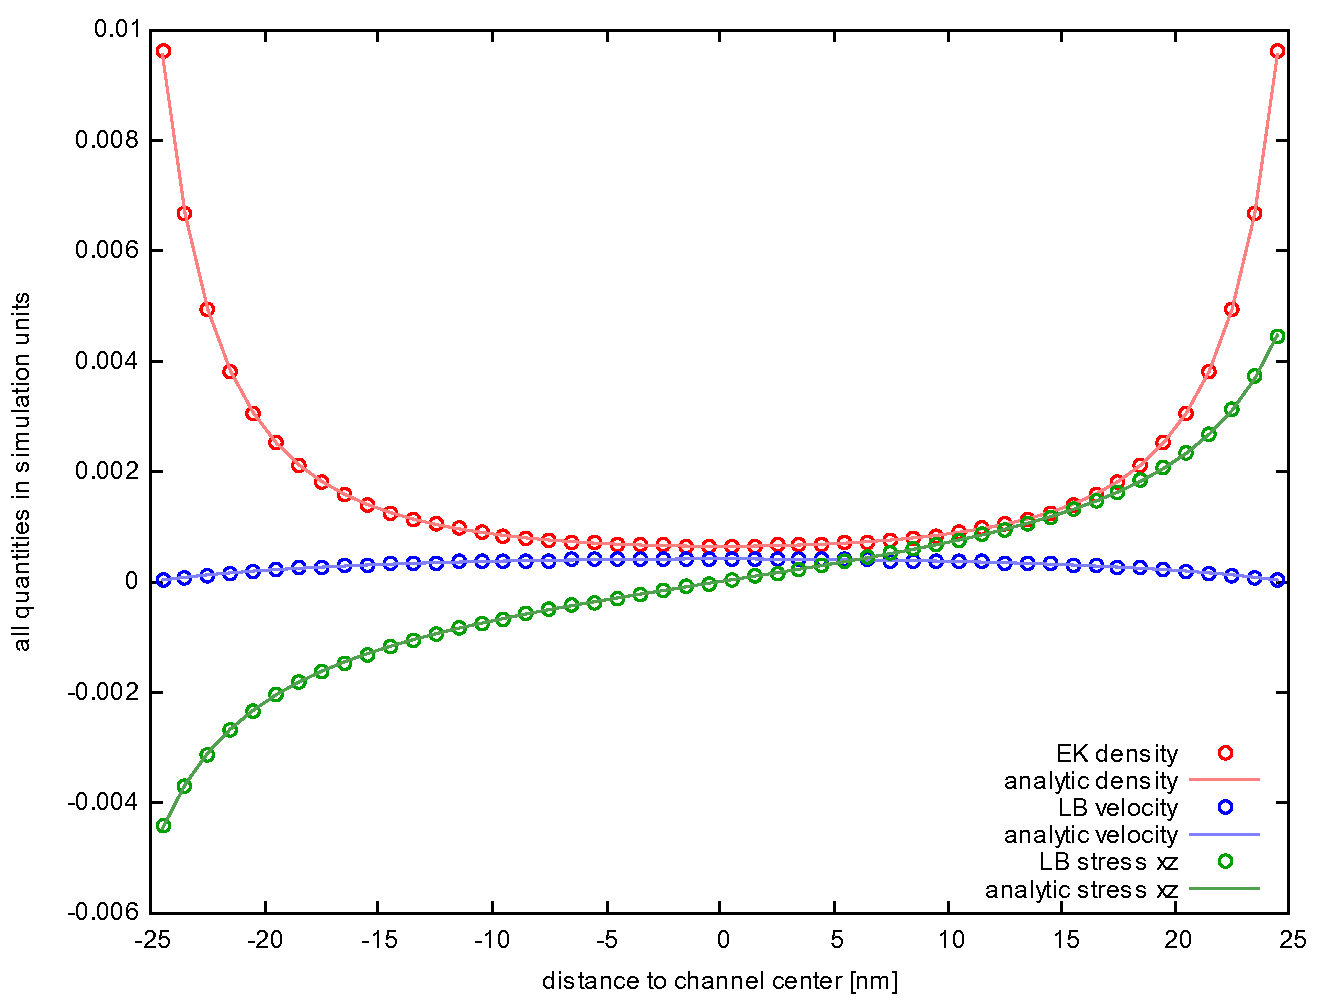
\includegraphics[width=1.0\columnwidth]{figures/profiles.pdf}
  \end{center}
  \caption{\label{fig:result}Profiles along the direction perpendicular to the slit pore walls for the counterion density, fluid velocity, and fluid shear stress. Parameters as chosen in Section~\ref{sec:units}.}
\end{figure}
